\documentclass{article}
\usepackage[margin=0.5in]{geometry}
%! begin preamble = tikz
\usepackage[utf8]{inputenc}
\usepackage{comment}
\usepackage{tikz}
\usepackage{pgfplots}
\usetikzlibrary{shapes}
\usetikzlibrary{3d}
\pgfplotsset{width=20cm, compat=1.18}
%! end preamble = tikz

\begin{document}

\pgfplotsset{visible stretch/.style={restrict expr to
domain={sin(atan2(rawy,rawx)-\pgfkeysvalueof{/pgfplots/view/az})}{-1.1:0}},hidden
stretch/.style={restrict expr to
domain={sin(atan2(rawy,rawx)-\pgfkeysvalueof{/pgfplots/view/az})}{0:1.1}}}
\def\addFGBGplot[#1]#2;{
    \addplot3[#1,hidden stretch, opacity=0.25] #2;
    \addplot3[#1,visible stretch] #2;
}

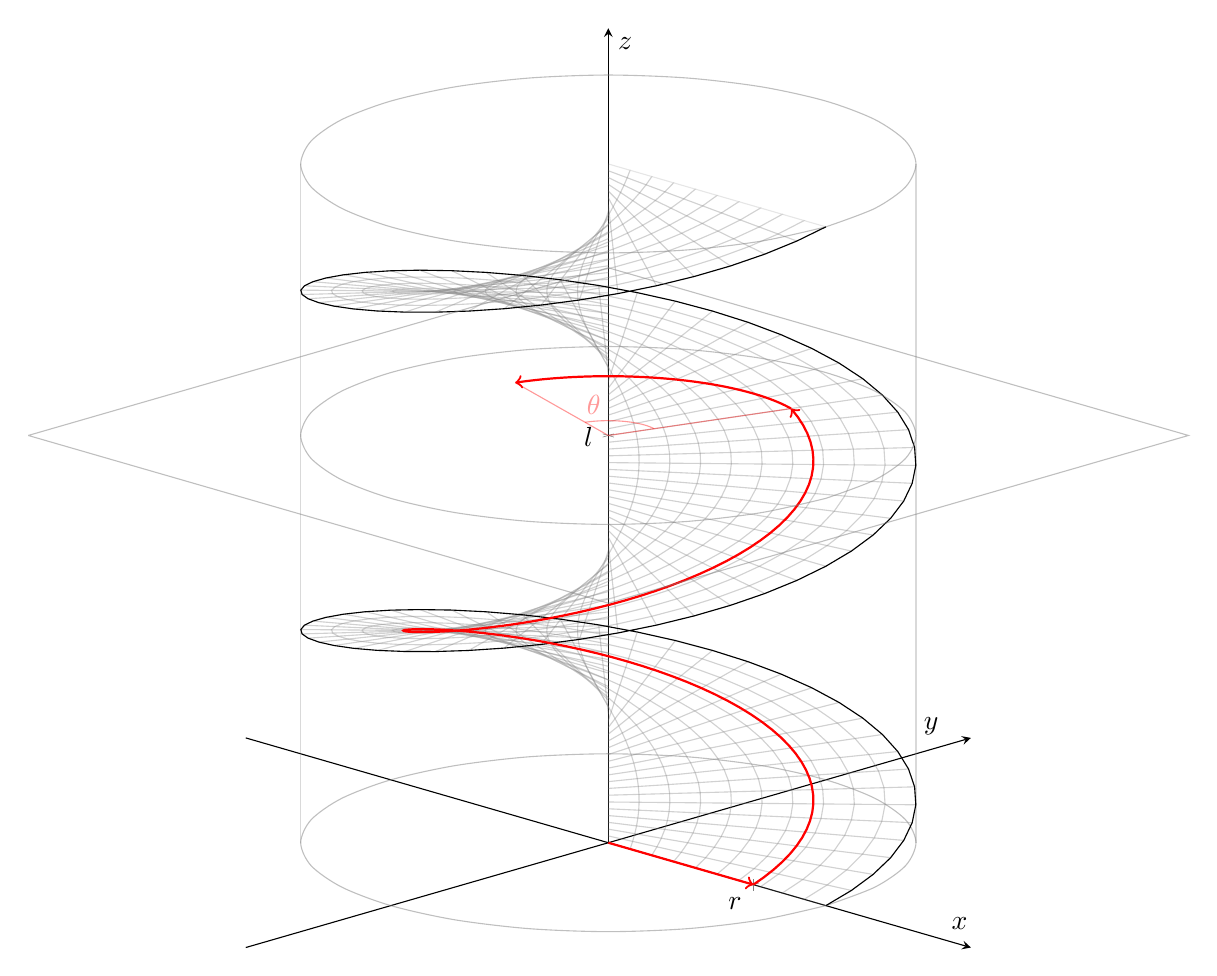
\begin{tikzpicture}[declare function={R=3;H=10;r=2;l=6;t=pi/2;}]
smallarrowhead/.style={
        ->,>={Latex[angle=60:3pt]},
    }
\begin{axis} [
    view={45}{20},
    axis lines = center,
    xlabel={$x$},
    ylabel={$y$},
    zlabel={$z$},
    xmin={-R-2},
    xmax={R+2},
    ymin={-R-2},
    ymax={R+2},
    zmax={H+2},
    xtick= {r},
    xticklabels = {$r$},
    ytick= {0},
    ztick= {l},
    zticklabels = {$l$},
]
% Cylinder
\addplot3[samples y=0,domain=0:360,smooth,draw=gray, opacity=0.5] ({R*cos(x)},{R*sin(x)},{H});
\addplot3[samples y=0,domain=0:360,smooth,draw=gray, opacity=0.5] ({R*cos(x)},{R*sin(x)},{0});
\draw[gray, opacity=0.3]  ({R*cos(\pgfkeysvalueof{/pgfplots/view/az})},{R*sin(\pgfkeysvalueof{/pgfplots/view/az})
 },{0}) -- ({R*cos(\pgfkeysvalueof{/pgfplots/view/az})},{R*sin(\pgfkeysvalueof{/pgfplots/view/az})},{H})
  ({R*cos(\pgfkeysvalueof{/pgfplots/view/az}-180)},{R*sin(\pgfkeysvalueof{/pgfplots/view/az}-180)
 },{0}) -- ({R*cos(\pgfkeysvalueof{/pgfplots/view/az}-180)},{R*sin(\pgfkeysvalueof{/pgfplots/view/az}-180)},{H});

% Helicoid
\addplot3[surf,
    color=gray,
    faceted color=gray,
    opacity=0.2,
    fill opacity=0,
    domain=0:H,
    domain y=0:R,
    samples=101,
    samples y=11,z buffer=sort
]
({y*cos(deg(4*pi/H*x))},
{y*sin(deg(4*pi/H*x))},
{x});
\addplot3[
    color=black,
    opacity=1,
    domain=0:H,
    samples=101,
    samples y=0,
]
({R*cos(deg(4*pi/H*x))},
{R*sin(deg(4*pi/H*x))},
{x});

% Point
\addplot3[
    color=red,
    ->,
    thick
] coordinates 
{
    (0,0,0)
    (r,0,0)
};
\addplot3[
    color=red,
    domain=0:l,
    samples=101,
    samples y=0,
    ->,
    thick
]
({r*cos(deg(4*pi/H*x))},
{r*sin(deg(4*pi/H*x))},
{x});
\addplot3[samples y=0,domain=0:t,smooth,draw=red, ->, thick] ({r*cos(deg(x + 4*pi/H*l)},{r*sin(deg(x + 4*pi/H*l))},{l});
\addplot3[samples y=0,domain=0:360,smooth,draw=gray, opacity=0.5] ({R*cos(x)},{R*sin(x)},{l});
\addplot3[
    draw=red, opacity=0.4
] coordinates 
{
    ({r*cos(deg(4*pi/H*l)},{r*sin(deg(4*pi/H*l))},l)
    (0,0,l)
    ({r*cos(deg(t + 4*pi/H*l)},{r*sin(deg(t + 4*pi/H*l))},l)
};
\addplot3[samples y=0,domain=0:t,smooth,draw=red, opacity=0.4] ({0.5*cos(deg(x + 4*pi/H*l)},{0.5*sin(deg(x + 4*pi/H*l))},{l});
\node at (-0.5,0.3,l+0.2) [red, opacity=0.4] {$\theta$};

% Plane
\addplot3[
    draw=gray, opacity=0.5
] coordinates 
{
    ({-R-1},{-R-1},l)
    ({-R-1},{+R+1},l)
    ({+R+1},{+R+1},l)
    ({+R+1},{-R-1},l)
    ({-R-1},{-R-1},l)
};


\end{axis}
\end{tikzpicture}

\end{document}